%% \documentclass{beamer}
\documentclass[fleqn]{beamer}

%% %-----------------------------------------------------
%% \usepackage{kotex} 
%% \setmainhangulfont[Mapping=tex-text]{NanumMyeongjo}   %% install ubuntu: Nanum Korean fonts
%% \setsanshangulfont[Mapping=tex-text]{NanumGothic}
%% \setmonohangulfont[Scale=0.95]{NanumGothicCoding}
%% %-----------------------------------------------------

\usepackage[english]{babel}
\usepackage{amsmath,amssymb}
\usepackage{chicago}
%======================================================


%======================================================
\setbeamertemplate{caption}[numbered]{}% Number float-like environments
\setbeamertemplate{theorems}[numbered] % Numbering for Theorem
\newenvironment<>{proofs}[1][\proofname]{%
    \par
    \def\insertproofname{#1{}}%
    \usebeamertemplate{proof begin}#2}
  {\usebeamertemplate{proof end}}
%======================================================
\setbeamercovered{transparent}
%% \colorlet{structure}{green!50!black}  
\mode<presentation>
{
  %% \setbeamertemplate{background canvas}[vertical shading][bottom=red!10,top=blue!10]
\usetheme{Madrid} %%\usecolortheme{beaver}
%%\usefonttheme{structuresmallcapsserif}
%%\usefonttheme[onlysmall]{structurebold}
}
\mode<article>{\usepackage{fullpage}}
% everybody
\usepackage{pgf}



%%=============================================================
\title[Weibullness]{Weibullness 
Test Using the Sample Correlation Coefficient with Probability Plots}
\author[Chanseok Park]{Chanseok Park}
\institute[Applied Statistics Lab.]%
{Applied Statistics Laboratory \\
Department of Industrial Engineering\\
Pusan National University}

\date{}
%% \date{\small Seminar Talk at Inje University, May 15, 2006\\
%% Host: Dr.\ Seong Beom Lee}
%%=============================================================


%==============================================================
\begin{document}
\begin{frame}
\titlepage
\vfill

\date{}

%% \centerline{\small\textsf{Hosted by SEC}}

\begin{center}
{
\includegraphics[scale=0.30]{PNU-logo3.jpg}}
\end{center}
\vfill
\end{frame}
%----------------------------------------------
%% \section<presentation>*{OVERVIEW}
\setcounter{tocdepth}{2}
\begin{frame}
  \frametitle{Overview}
     \tableofcontents[pausesections]
\end{frame}
%%============================================================================


%%============================================================================
%% \part<presentation>{Main Talk}
%%============================================================================
    


 %%===============================================================
 \clearpage
 \section[Weibull Plots]{Weibull Plots}
 %--------------------
 %----------------------------------------------------
\subsection{Weibull random variable}
%----------------------------------------------------

\begin{frame}
\frametitle{Weibull random variable}
\begin{itemize}
\item One of the most popular distributions used to model the lifetimes and reliability data
is the Weibull distribution, named after a Swedish \textbf{mechanical engineer} by the name of
Walodie Weibull~\citeyear{Weibull:1939}.
\item Indeed, this distribution is as central to the parametric analysis of 
\textbf{reliability engineering} and \textbf{survival} data as the normal distribution in statistics.
\end{itemize}
\end{frame}

%------
\begin{frame}
\frametitle{Weibull random variable}
\begin{block}{Definition}
A random variable $X$ is called \textsf{Weibull} with shape $\alpha$
and scale $\beta$
if its cumulative distribution function is given by
$$
F(x) = 1 - \exp\Big\{ - \big( \frac{x}{\beta} \big)^{\alpha}   \Big\},
\qquad x \ge 0.
$$
\end{block}
It is easily shown that its pdf is given by
$$
f(x) =  \frac{\alpha x^{\alpha-1}}{\beta^\alpha} 
        \exp\Big\{ - \big( \frac{x}{\beta} \big)^{\alpha} \Big\}.
$$
The mean of the Weibull random variable is
$\beta\cdot\Gamma\big[ (\alpha+1)/\alpha \big]$, where
$\Gamma(\alpha)=\int_0^{\infty} x^{\alpha-1} e^{-x} dx$.
\end{frame}
%------

%------
\begin{frame}
\frametitle{Weibull random variable}
\begin{block}{Reparameterized Form}
The following reparameterized form is often used
%---------
\begin{align*}
F(x) = 1 - \exp\big( - \lambda x^{\alpha}  \big)  \textrm{~~and~~} 
f(x) = \lambda\alpha x^{\alpha-1} \exp\big( - \lambda x^{\alpha}  \big),
\end{align*}
\end{block}
%---------
where $\lambda=\beta^{-\alpha}$. 
\begin{itemize}
\item The parameter $\lambda$ is called the \textsf{rate parameter}\index{rate parameter}.
\item It should be noted that with the shape parameter $\alpha=1$, the Weibull distribution
becomes the exponential distribution\index{exponential distribution}
with mean $\beta$ (or rate $\lambda$).
\end{itemize}
\end{frame}
%------


%----------------------------------------------------
\subsection{How to draw Weibull probability plot}
%----------------------------------------------------

%------
\begin{frame}
\frametitle{How to draw Weibull probability plot}

{\Large\bf Basic Idea:} Linearizing the CDF.

\end{frame}
%------

%------
\begin{frame}
\frametitle{How to draw Weibull probability plot}
The Weibull cdf is given by
$$
F(x) = 1 - \exp\big( - \lambda x^{\alpha}  \big). 
$$
Then we have
$$
\log(1-p) = -\lambda x_p^{\alpha}, 
$$
where $p=F(x)$. It follows that
$$
\log\big\{ -\log(1-p) \big\} = \log\lambda + \alpha \log x_p.
$$
This implies that the plot of  
\begin{block}{}
\begin{center}
\fbox{$\log\big\{ -\log(1-p) \big\}$} versus \fbox{$\log x_p$} 
\end{center}
\end{block}
draws a straight line with the slope $\alpha$ and the intercept $\log\lambda$.
The widely-used Weibull \textit{probability paper}\index{probability paper}
is based on this idea.
\end{frame}
%------



\begin{frame}
\frametitle{How to draw Weibull probability plot}
\begin{itemize}
\item Need to find $p=F(x)$ and $x_p$ with real experimental data. 
That is, we need to estimate  $p=F(x)$ and $x_p$ in the following plot:
\item The empirical cdf $\hat{F}(x)$ is used for $p=F(x)$ which is an increasing
 step function jumping $1/n$ at
$x_{(1)}, x_{(2)}, \ldots, x_{(n)}$, where $x_{(i)}$ is sorted from the smallest. 
\item Thus $\hat{p}_i=\hat{F}(x_{(i)})$ has values, $1/n, 2/n, \ldots, n/n$. 

\begin{block}{}
\begin{center}
\fbox{$\log\big\{ -\log(1- \hat{p}_i ) \big\}$} versus \fbox{$\log x_{(i)} $}.
\end{center}
\end{block}
 Actually, \cite{Blom:1958} method is more popular, which uses 
$\hat{p}_i= (i-0.375)/(n+0.25)$ to have better power -- plotting position problem.
\end{itemize}
\end{frame}
%------



 %%===============================================================
 \clearpage
 \section[Examples]{Weibull Plot Examples}
 %--------------------
 %=================================================================
\subsection{Example 1: W-LN}
%=================================================================
\begin{frame}
  \frametitle{Example 1: W-LN}

\begin{footnotesize}
\begin{block}{Data I}
1.208339 1.748644 2.080409 2.335513 2.548681 2.734928 2.902281
3.055600 3.198078 3.331945 3.458826 3.579955 3.696291 3.808603
3.917520 4.023568 4.127191 4.228776 4.328661 4.427151 4.524519
4.621021 4.716894 4.812366 4.907658 5.002987 5.098571 5.194633
5.291403 5.389125 5.488057 5.588484 5.690718 5.795109 5.902057
6.012024 6.125552 6.243292 6.366035 6.494765 6.630734 6.775576
6.931493 7.101568 7.290332 7.504885 7.757387 8.071660 8.506590
9.315591
\end{block}

\begin{block}{Data II}
\begin{color}{red}
2.132357  2.451394  2.652611  2.809841  2.943303  3.061764  3.169903
 3.270548  3.365555  3.456222  3.543500  3.628113  3.710634  3.791524
 3.871172  3.949906  4.028015  4.105758  4.183369  4.261071  4.339071
 4.417576  4.496786  4.576906  4.658146  4.740724  4.824872  4.910837
 4.998892  5.089334  5.182497  5.278755  5.378541  5.482349  5.590762
 5.704470  5.824303  5.951271  6.086630  6.231970  6.389342  6.561469
 6.752075  6.966453  7.212504  7.502789  7.859157  8.324999  9.008337
10.356137
\end{color}
\end{block}
\end{footnotesize}
%----------
\end{frame}

%% %%--------------------------------
\begin{frame}   %%[allowframebreaks]
\begin{figure}[h]
   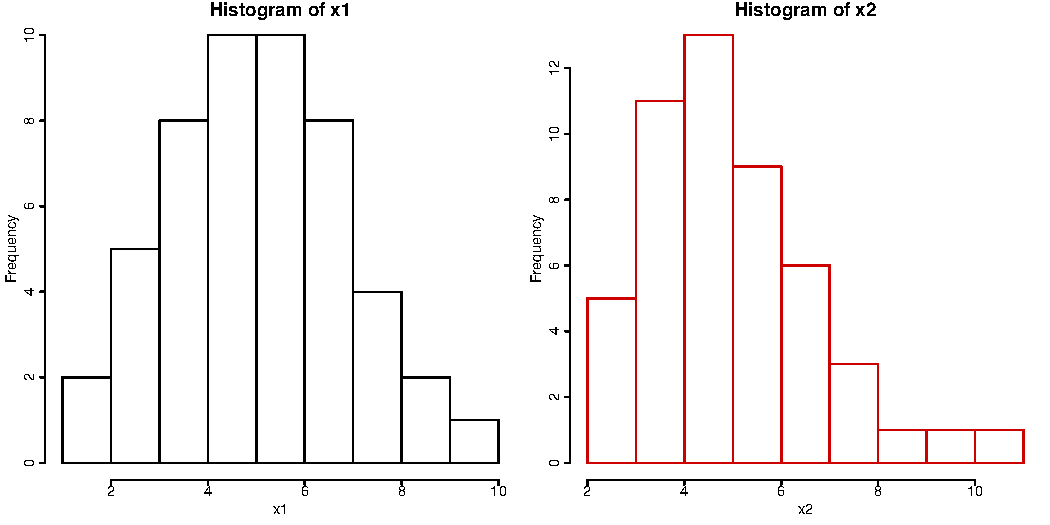
\includegraphics[width=4.5in]{hist1.pdf} %%-Figure (pdf file)
   \vspace{-3ex}
\end{figure}
\end{frame}
%% %%--------------------------------
% \begin{frame}   %%[allowframebreaks]
% \begin{figure}[h]
% %%  %% \centering\includegraphics{BPweibullplot.ps} %%-Figure (ps file)
%    \includegraphics[height=4.5in,angle=90]{CDF1a.pdf} %%-Figure (pdf file)
%    \vspace{-3ex}
% \end{figure}
% \end{frame}
% %% %%--------------------------------
% \begin{frame}   %%[allowframebreaks]
% \begin{figure}[h]
% %%  %% \centering\includegraphics{BPweibullplot.ps} %%-Figure (ps file)
%    \includegraphics[height=3.0in,angle=90]{CDF1b.pdf} %%-Figure (pdf file)
%    \vspace{-3ex}
% \end{figure}
% \end{frame}
%% %%---------------------------------------------------
\begin{frame}   %%[allowframebreaks]
\begin{figure}[h]
%%  %% \centering\includegraphics{BPweibullplot.ps} %%-Figure (ps file)
   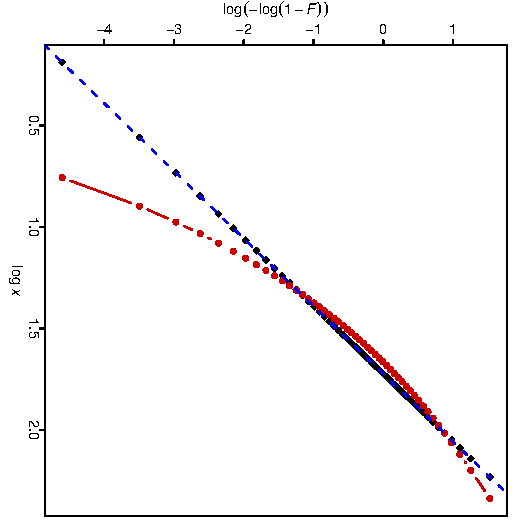
\includegraphics[width=3.0in,angle=90]{Weibull1.pdf} %%-Figure (pdf file)
   \vspace{-3ex}
\end{figure}
\end{frame}
%% %%---------------------------------------------------


 %=================================================================
\subsection{Example 2: W-N}
%=================================================================
\begin{frame}
  \frametitle{Example 2: W-N}

\begin{footnotesize}
\begin{block}{Data I}
1.208339 1.748644 2.080409 2.335513 2.548681 2.734928 2.902281
3.055600 3.198078 3.331945 3.458826 3.579955 3.696291 3.808603
3.917520 4.023568 4.127191 4.228776 4.328661 4.427151 4.524519
4.621021 4.716894 4.812366 4.907658 5.002987 5.098571 5.194633
5.291403 5.389125 5.488057 5.588484 5.690718 5.795109 5.902057
6.012024 6.125552 6.243292 6.366035 6.494765 6.630734 6.775576
6.931493 7.101568 7.290332 7.504885 7.757387 8.071660 8.506590
9.315591
\end{block}

\begin{block}{Data II}
\begin{color}{red}
0.923350 1.642687 2.049681 2.346765 2.586173 2.789748 2.968822
3.130079 3.277814 3.414961 3.543624 3.665370 3.781399 3.892659
3.999913 4.103790 4.204817 4.303443 4.400057 4.495004 4.588591
4.681098 4.772786 4.863899 4.954671 5.045329 5.136101 5.227214
5.318902 5.411409 5.504996 5.599943 5.696557 5.795183 5.896210
6.000087 6.107341 6.218601 6.334630 6.456376 6.585039 6.722186
6.869921 7.031178 7.210252 7.413827 7.653235 7.950319 8.357313
9.076650
\end{color}
\end{block}
\end{footnotesize}
%----------
\end{frame}


%% %%--------------------------------
\begin{frame}   %%[allowframebreaks]
\begin{figure}[h]
   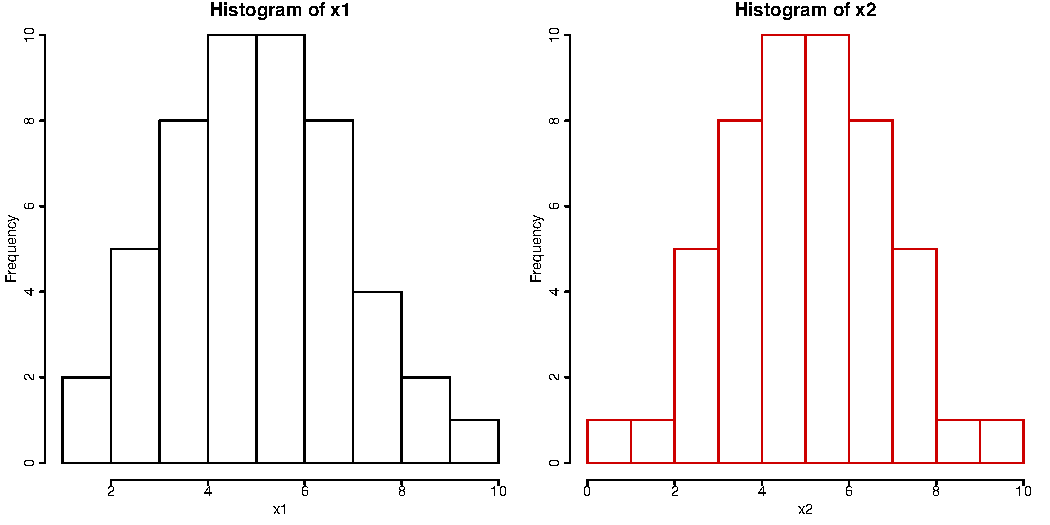
\includegraphics[width=4.5in]{hist2.pdf} %%-Figure (pdf file)
   \vspace{-3ex}
\end{figure}
\end{frame}
%% %%--------------------------------
% \begin{frame}   %%[allowframebreaks]
% \begin{figure}[h]
% %%  %% \centering\includegraphics{BPweibullplot.ps} %%-Figure (ps file)
%    \includegraphics[height=4.5in,angle=90]{CDF2a.pdf} %%-Figure (pdf file)
%    \vspace{-3ex}
% \end{figure}
% \end{frame}
% %% %%--------------------------------
% \begin{frame}   %%[allowframebreaks]
% \begin{figure}[h]
% %%  %% \centering\includegraphics{BPweibullplot.ps} %%-Figure (ps file)
%    \includegraphics[height=3.0in,angle=90]{CDF2b.pdf} %%-Figure (pdf file)
%    \vspace{-3ex}
% \end{figure}
% \end{frame}
%% %%---------------------------------------------------
\begin{frame}   %%[allowframebreaks]
\begin{figure}[h]
%%  %% \centering\includegraphics{BPweibullplot.ps} %%-Figure (ps file)
   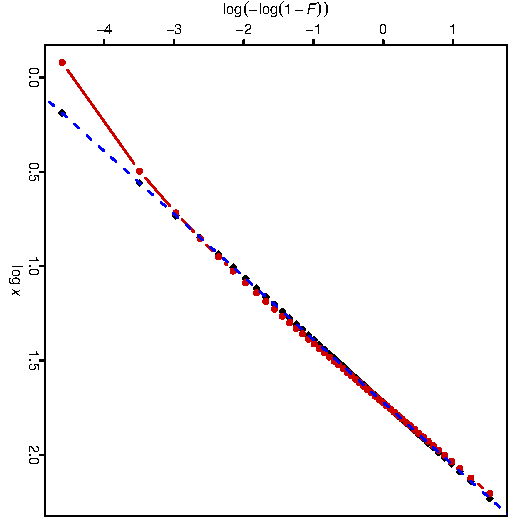
\includegraphics[width=3.0in,angle=90]{Weibull2.pdf} %%-Figure (pdf file)
   \vspace{-3ex}
\end{figure}
\end{frame}
%% %%---------------------------------------------------


 %=================================================================
\subsection{Example 3: W-W}
%=================================================================
\begin{frame}
  \frametitle{Example 3: W-W}
%%\vspace*{-5pt}
\begin{footnotesize}
\begin{block}{Data I}
1.208339 1.748644 2.080409 2.335513 2.548681 2.734928 2.902281
3.055600 3.198078 3.331945 3.458826 3.579955 3.696291 3.808603
3.917520 4.023568 4.127191 4.228776 4.328661 4.427151 4.524519
4.621021 4.716894 4.812366 4.907658 5.002987 5.098571 5.194633
5.291403 5.389125 5.488057 5.588484 5.690718 5.795109 5.902057
6.012024 6.125552 6.243292 6.366035 6.494765 6.630734 6.775576
6.931493 7.101568 7.290332 7.504885 7.757387 8.071660 8.506590
9.315591
\end{block}

%% \vspace*{-5pt}
\begin{block}{Data II}
\begin{color}{red}
 0.0502516  0.1522960  0.2564664  0.3628534  0.4715534
 0.5826690  0.6963103  0.8125946  0.9316478  1.0536051
 1.1786116  1.3068238  1.4384103  1.5735537  1.7124515
 1.8553184  2.0023878  2.1539145  2.3101773  2.4714816
 2.6381637  2.8105945  2.9891850  3.1743913  3.3667227
 3.5667494  3.7751129  3.9925384  4.2198503  4.4579906
 4.7080427  4.9712613  5.2491106  5.5433131  5.8559149
 6.1893717  6.5466666  6.9314718  7.3483798  7.8032387
 8.3036560  8.8597842  9.4855999 10.2011041 11.0363745
12.0397280 13.2963001 14.9786613 17.5327894 23.0258509
\end{color}
\end{block}
\end{footnotesize}
%----------
\end{frame}


%% %%--------------------------------
\begin{frame}   %%[allowframebreaks]
\begin{figure}[h]
   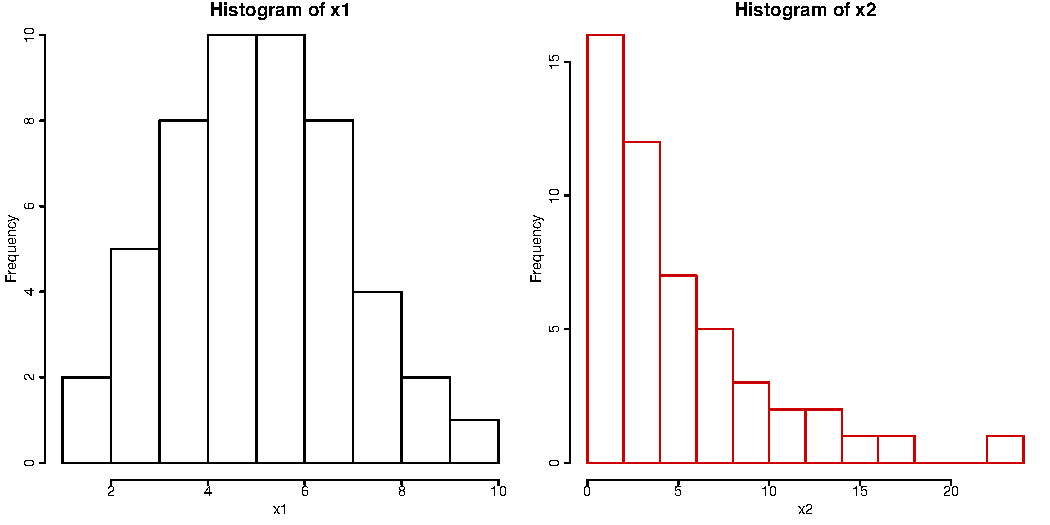
\includegraphics[width=4.5in]{hist3.pdf} %%-Figure (pdf file)
%%   \vspace{-3ex}
\end{figure}
\end{frame}
% %% %%--------------------------------
% \begin{frame}   %%[allowframebreaks]
% \begin{figure}[h]
% %%  %% \centering\includegraphics{BPweibullplot.ps} %%-Figure (ps file)
%    \includegraphics[height=4.5in,angle=90]{CDF3a.pdf} %%-Figure (pdf file)
%    \vspace{-3ex}
% \end{figure}
% \end{frame}
% %% %%--------------------------------
% \begin{frame}   %%[allowframebreaks]
% \begin{figure}[h]
% %%  %% \centering\includegraphics{BPweibullplot.ps} %%-Figure (ps file)
%    \includegraphics[height=3.0in,angle=90]{CDF3b.pdf} %%-Figure (pdf file)
%    \vspace{-3ex}
% \end{figure}
% \end{frame}
%% %%---------------------------------------------------
\begin{frame}   %%[allowframebreaks]
\begin{figure}[h]
%%  %% \centering\includegraphics{BPweibullplot.ps} %%-Figure (ps file)
   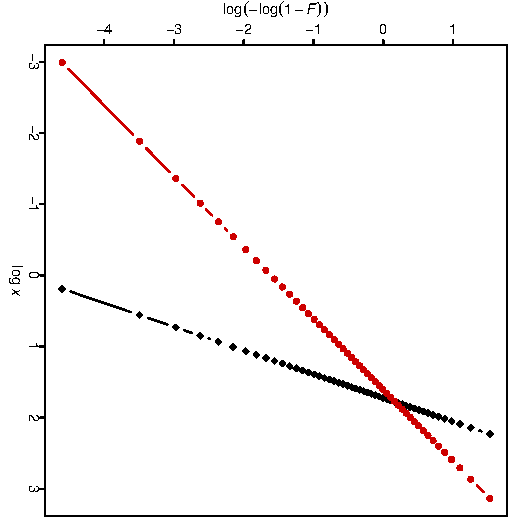
\includegraphics[width=3.0in,angle=90]{Weibull3.pdf} %%-Figure (pdf file)
   \vspace{-3ex}
\end{figure}
\end{frame}
%% %%---------------------------------------------------



 %%===============================================================
 \clearpage
 \section[Weibullness]{Test of Weibullness}
 %--------------------
 %=================================================================
\subsection{Real Data Example}
%=================================================================
\begin{frame}
  \frametitle{Birnbaum-Saunders and Leemis Real Data}
\begin{footnotesize}
\begin{block}{Data I  - from \citeN{Birnbaum/Saunders:1969b} }
\begin{color}{red}
0.07, 0.09, 0.096, 0.097, 0.099, 0.1, 0.103, 0.104, 0.104,
0.105, 0.107, 0.108, 0.108, 0.108, 0.109, 0.109, 0.112, 0.112,
0.113, 0.114, 0.114, 0.114, 0.116, 0.119, 0.12, 0.12, 0.12, 0.121,
0.121, 0.123, 0.124, 0.124, 0.124, 0.124, 0.124, 0.128, 0.128,
0.129, 0.129, 0.13, 0.13, 0.13, 0.131, 0.131, 0.131, 0.131, 0.131,
0.132, 0.132, 0.132, 0.133, 0.134, 0.134, 0.134, 0.134, 0.134,
0.136, 0.136, 0.137, 0.138, 0.138, 0.138, 0.139, 0.139, 0.141,
0.141, 0.142, 0.142, 0.142, 0.142, 0.142, 0.142, 0.144, 0.144,
0.145, 0.146, 0.148, 0.148, 0.149, 0.151, 0.151, 0.152, 0.155,
0.156, 0.157, 0.157, 0.157, 0.157, 0.158, 0.159, 0.162, 0.163,
0.163, 0.164, 0.166, 0.166, 0.168, 0.170, 0.174, 0.196, 0.212
\end{color}
\end{block}

\begin{block}{Data II - Example 8.16 in \citeN{Leemis:1995}}
17.88, 28.92, 33.00, 41.52, 45.12, 45.60, 48.48, 51.84, 51.96,
         54.12, 55.56, 67.80, 68.64, 68.64, 68.88, 84.12, 93.12, 98.64,
        105.12, 105.84, 127.92, 128.04, 173.40
\end{block}
\end{footnotesize}
%----------
\end{frame}

%% %%--------------------------------
\begin{frame}   %%[allowframebreaks]
\begin{figure}[h]
   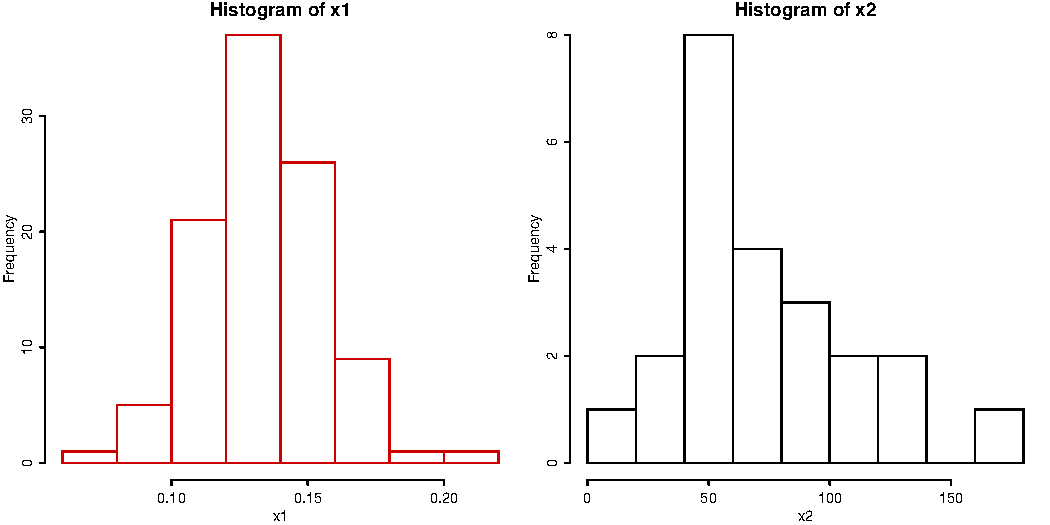
\includegraphics[width=4.5in]{hist4.pdf} %%-Figure (pdf file)
   \vspace{-3ex}
\end{figure}
\end{frame}

%% %%---------------------------------------------------
\begin{frame}   %%[allowframebreaks]
\begin{figure}[h]
   %%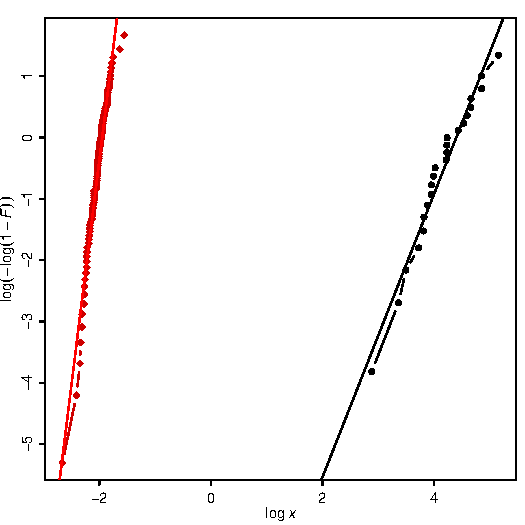
\includegraphics[width=3.0in,angle=90]{Weibull4.pdf} %%-Figure (pdf file)
   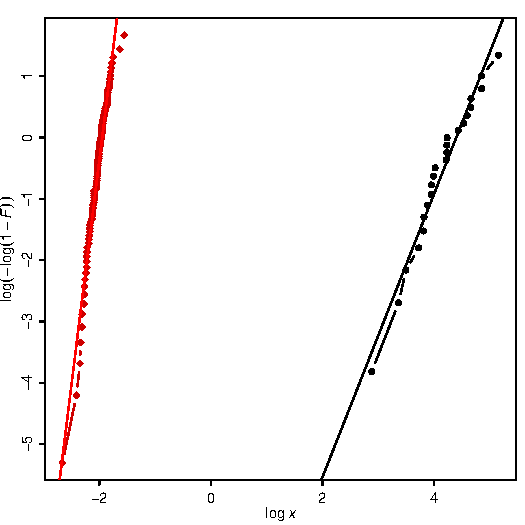
\includegraphics[width=3.0in]{Weibull4.pdf} %%-Figure (pdf file)
   \vspace{-3ex}
\end{figure}
\end{frame}
%% %%---------------------------------------------------



%% %%---------------------------------------------------
\begin{frame}   %%[allowframebreaks]
\begin{block}{How to determine whether the data are from Weibull or not}
\( \qquad
H_0: \text{Weibull}   \mathrm{~~versus~~}   H_1: \text{non-Weibull}  \)
\end{block}
\begin{itemize}
\item Recall: $\log\big\{ -\log(1-p) \big\} = \log\lambda + \alpha \log x_p.$
\item Thus \fbox{$\log\big\{ -\log(1-\hat{p}_i) \big\}$} versus \fbox{$\log x_{(i)}$}
draws a straight line, where $\hat{p}_i= (i-0.375)/(n+0.25)$.
Thus, the linearity measure (sample correlation) can be used for Weibullness test.
\item Idea: Large $r$ implies Weibullness.
\[ \boxed{  H_0: r \ge r_0  \mathrm{~~versus~~} H_1:  r < r_0 } \]
  Then,  how large is large enough for $r$? 
\item To this end, we should know the distribution of $r$ and then find the critical value
(from pivot) with the significance level (or Type-I error).
\end{itemize} 
\end{frame}
%% %%---------------------------------------------------


%% %%---------------------------------------------------
\begin{frame}   %%[allowframebreaks]
\begin{block}{Distribution of \(r\) sample correlations under the normal distribution}
If $(X,Y)$ is from bi-variate normal, it is known that 
\[  r\sqrt{ \frac{n-2}{1-r^2} } \sim t\text{-distribution} \]
with $n-2$ degrees of freedom.
\begin{itemize}
\item In general, $-1 \le r \le 1$, and $ -\infty < r\sqrt{\frac{n-2}{1-r^2}} < \infty$.
\item As $n \to \infty$, CLT works in general. 
      I.e., $r\sqrt{ \frac{n-2}{1-r^2} } \stackrel{d}{\to}N(0,1) $
\item In the Weibull plot,  $ 0 <  r \le 1$. 
      Thus, $0 < r\sqrt{\frac{n-2}{1-r^2}} < \infty$.
\item CLT can not work for the Weibull case.
\end{itemize}
\end{block}\end{frame}
%% %%---------------------------------------------------

%% %%---------------------------------------------------
\begin{frame}   %%[allowframebreaks]
\begin{itemize}
\item We can not use normal approximation. We need to find the distribution of $r$.
\item We can find the distribution of $r$ under Weibull distribution using Monte Carlo simulation. \\
\item Again, recall $\log\big\{ -\log(1-p) \big\} = \log\lambda + \alpha \log x_p.$ \\
\item Since $\mathrm{cor}(aX+b,cY+d) = \mathrm{cor}(X,Y)$, it is enough to generate random sample
of size $n$ from any Weibull distribution.
 This implies that the correlation 
from the Weibull plot is independent of the parameters $\alpha$ and $\lambda$.
\item Thus, the sample correlation is a \textbf{pivotal quantity}.
\end{itemize}
\end{frame}
%----------
\begin{frame}  
\begin{block}{Algorithm}
\begin{itemize}
\item Generate Weibull random observations of size $n$ from any Weibull, say, Weibull (1,1).
\item Sort the data. Denote $x_{(i)}$.
\item Calculate $\log\big\{ -\log(1-\hat{p}_i) \big\}$ where $\hat{p}_i= (i-0.375)/(n+0.25)$.
\item Calculate the sample correlation between $\log\big\{ -\log(1-\hat{p}_i) \big\}$ and $\log x_{(i)}$.
\item Repeat the above (say, up to $N$ iteration numbers).
\item Find the empirical quantiles for critical values (say, 5\%, 10\%, etc.)
\end{itemize}
\end{block}\end{frame}




%% %%---------------------------------------------------
\begin{frame}   %%[allowframebreaks]
\begin{figure}[h]
   %%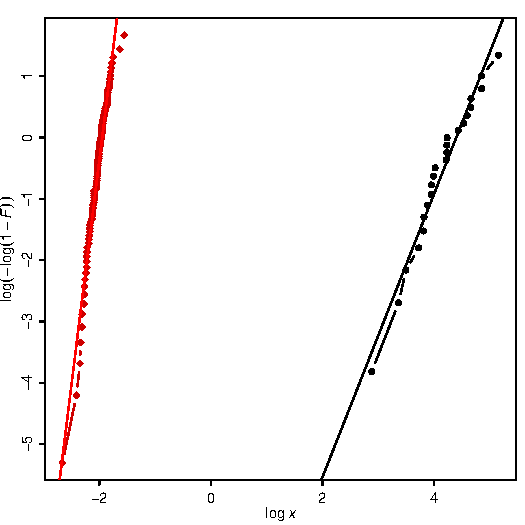
\includegraphics[width=3.0in,angle=90]{Weibull4.pdf} %%-Figure (pdf file)
   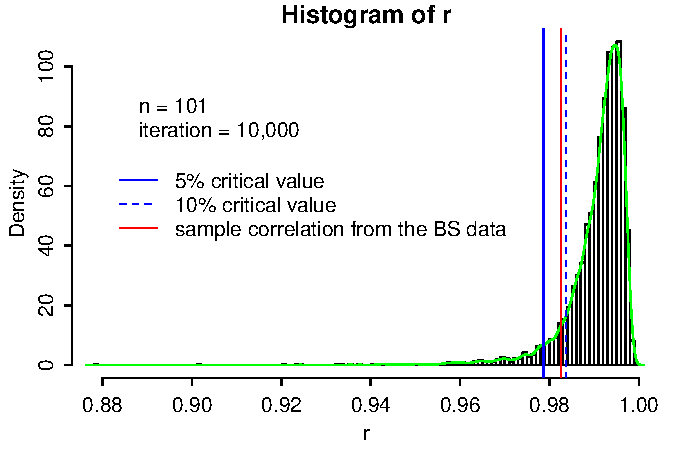
\includegraphics[width=4.5in]{hist-corr1.pdf} %%-Figure (pdf file)
   \vspace{-3ex}
\end{figure}
\end{frame}
%% %%---------------------------------------------------



%% %%---------------------------------------------------
\begin{frame}   %%[allowframebreaks]
\begin{figure}[h]
   %%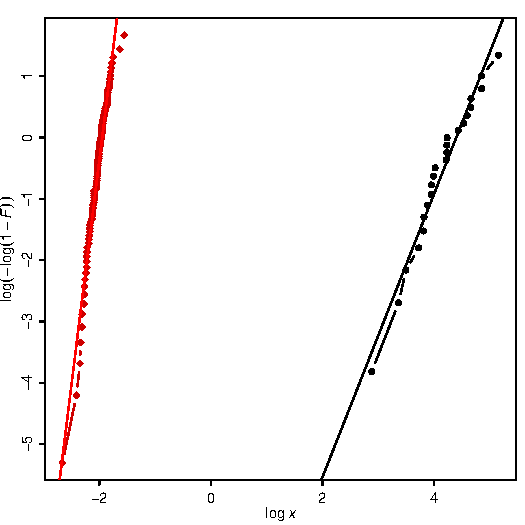
\includegraphics[width=3.0in,angle=90]{Weibull4.pdf} %%-Figure (pdf file)
   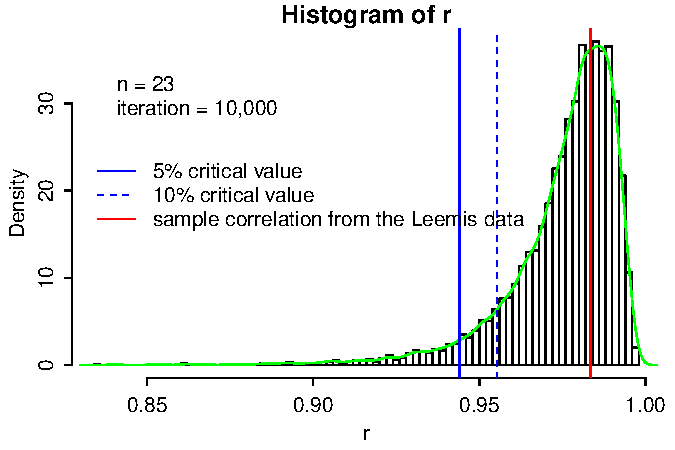
\includegraphics[width=4.5in]{hist-corr2.pdf} %%-Figure (pdf file)
   \vspace{-3ex}
\end{figure}
\end{frame}
%% %%---------------------------------------------------






%% %%---------------------------------------------------
\begin{frame}   %%[allowframebreaks]
\begin{block}{Critical Values}
\begin{tabular}{cccccccc}
\hline
$n$ & &1.0\%  &2.0\%  &2.5\%  &5.0\%  &10\%   &20\%  \\
\hline
101 & &0.9593 &0.9686 &0.9710 &\textcolor{red}{0.9777} & \textcolor{red}{0.9833} &0.9878 \\
 23 & &0.9085 &0.9239 &0.9284 &0.9429 &0.9553 &0.9665 \\
\hline
\end{tabular}
\end{block}

\begin{block}{Sample Correlations for the BS and Leemis Data Sets}
\begin{itemize}
\item Data I (BS Data) \\
$r = \textcolor{red}{0.982614}$ with $n=101$ \\
Using 5\% Type-I error, the Data are from Weibull.
With 10\% or more Type-I error, the Data are not from Weibull.
\item Data II (Leemis Data) \\
$r = 0.983456$ with $n=23$ \\
The Data are from Weibull for any above Type-I errors.
\end{itemize}
\end{block}
We can also find the $p$-value from the empirical pdf.
The $p$-value for the BS data is 8.5\% while that for the Leemis is 63\%.
\end{frame}
%% %%---------------------------------------------------


%% %%---------------------------------------------------
\begin{frame}   %%[allowframebreaks]
\begin{figure}[h]
   %%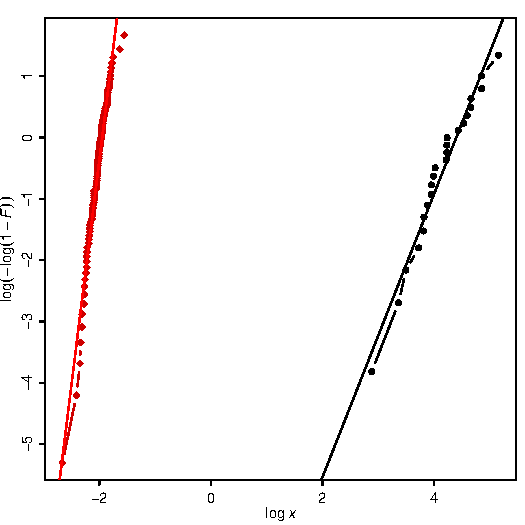
\includegraphics[width=3.0in,angle=90]{Weibull4.pdf} %%-Figure (pdf file)
   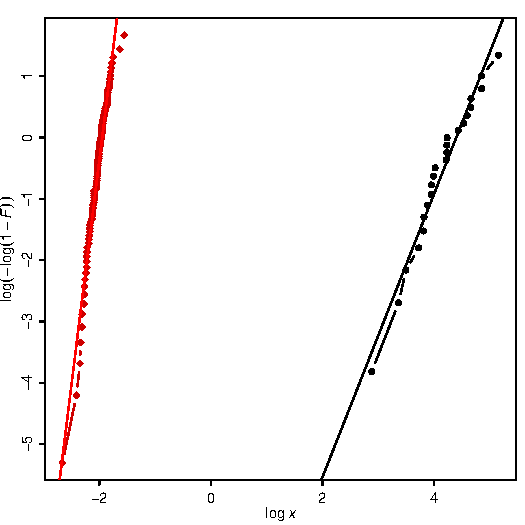
\includegraphics[width=3.0in]{Weibull4.pdf} %%-Figure (pdf file)
   \vspace{-3ex}
\end{figure}
\end{frame}
%% %%---------------------------------------------------


%=================================================================
\subsection{Weibullness R Package}
%=================================================================
%% %%---------------------------------------------------
\begin{frame}[fragile]{Weibullness R Package}
Testing Weibullness can be easily performed by using \texttt{weibullness} R package
\cite{Park:2018b}. 
One can refer to:
\begin{itemize}
\item \url{https://appliedstat.github.io/R/R-package-1/}  \\
     \href{https://appliedstat.github.io/R/R-package-1/}{\beamergotobutton{Link}}
\item \url{https://cran.r-project.org/web/packages/weibullness/}  \\
     \href{https://cran.r-project.org/web/packages/weibullness/}{\beamergotobutton{Link}}
\end{itemize}
\begin{exampleblock}{Installation}
\begin{verbatim}
> install.packages("weibullness")

> library("weibullness")
> help(package="weibullness")
\end{verbatim}
\end{exampleblock}
\end{frame}









%%
%%
%%


%%==================================================================
   \begin{frame}[allowframebreaks]
    \frametitle{References}
%%  \beamertemplatebookbibitems

%% \bibliographystyle{apalike}
   \bibliographystyle{chicago}
%% \bibliographystyle{unsrt}
%% \bibliographystyle{plain}
%% \bibliographystyle{natbib} 
%% \bibliographystyle{$HOME/library/TeX/natbib/natbib} 
%%%   \bibliography{$HOME/MyFiles/library/TeX/bib/STAT,% 
%%%$HOME/MyFiles/library/TeX/bib/CP,% 
%%%$HOME/MyFiles/library/TeX/bib/ENG}

\begin{thebibliography}{}

\bibitem[\protect\citeauthoryear{Birnbaum and Saunders}{Birnbaum and
  Saunders}{1969}]{Birnbaum/Saunders:1969b}
Birnbaum, Z.~W. and S.~C. Saunders (1969).
\newblock Estimation for a family of life distributions with applications to
  fatigue.
\newblock {\em Journal of Applied Probability\/}~{\em 6}, 328--347.

\bibitem[\protect\citeauthoryear{Blom}{Blom}{1958}]{Blom:1958}
Blom, G. (1958).
\newblock {\em Statistical Estimates and Transformed Beta Variates}.
\newblock New York: Wiley.

\bibitem[\protect\citeauthoryear{Leemis}{Leemis}{1995}]{Leemis:1995}
Leemis, L.~M. (1995).
\newblock {\em Reliability}.
\newblock Englewood Cliffs, N.J.: Prentice-Hall.

\bibitem[\protect\citeauthoryear{Park}{Park}{2018}]{Park:2018b}
Park, C. (2018).
\newblock \texttt{weibullness}: Goodness-of-fit test for {W}eibull
  ({W}eibullness test).
\newblock \url{https://CRAN.R-project.org/package=weibullness}.
\newblock R package version 1.18.6.

\bibitem[\protect\citeauthoryear{Weibull}{Weibull}{1939}]{Weibull:1939}
Weibull, W. (1939).
\newblock A statistical theory of the strength of material.
\newblock {\em Proceedings, Royal Swedish Institute for Engineering
  Research\/}~{\em 151}, 1--45.

\end{thebibliography}
   \end{frame}
%%==================================================================  


%%====================================================================
\end{document}
%%====================================================================

